\subsection{Data Transfer Object Pattern}
\label{data_transfer_object_pattern_section}

It is a well-known fact that many small requests between two processes, and even
more between two hosts in a network need a lot of time. The local machine with
two processes has to permanently exchange the program context and the network
has a lot of transfers. For each request, there is at least a necessity of two
transfers -- the question of the client and the answer of the server.\\
Transfer-methods are often expected to deliver common data such as a Person's
address, i.e. surname, first name, street, zip-code, town etc. These information
is best retrieved by only one transfer-call. That way, the client has to wait
only once for a server response and the server does not get too many single tasks.
In the address-example, all address data would best be packaged together and
sent back to the client.

\begin{figure}[ht]
    \begin{center}
       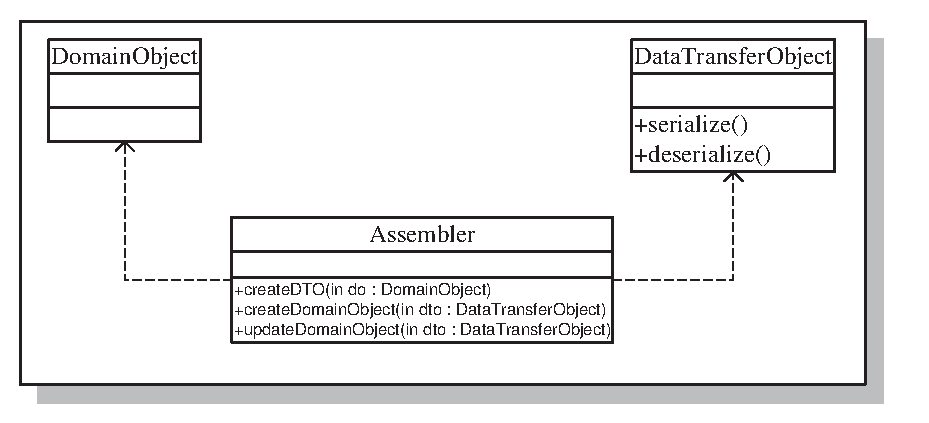
\includegraphics[scale=0.5]{images/data_transfer_object_pattern.eps}
       \caption{The Data Transfer Object - Pattern \cite{enterprisepattern}}
       \label{datatransferobject_figure}
    \end{center}
\end{figure}

And that is exactly what the Data Transfer Object pattern (figure \ref{datatransferobject_figure})
proposes a solution for: A central \emph{Assembler} class takes all common data
of the server's domain model object and assembles them together into a special
object called \emph{Data Transfer Object} (DTO) which is a flat data structure.
The server will then send this DTO over network to the client. On the client's side,
a similar assembler takes the DTO, finds out all received data and maps (disassembles) them to the
client's domain model. In that manner, a DTO is able to drastically improve the performance
in communications.\\
Comparing with the Data Mapper from chapter \ref{data_mapper_pattern_section},
the assembler's task of translating between data models seems quite similar if
not the same. Hence, why shouldn't it be possible for inter-system-communications
over network to use a \emph{Translator} similar to the one for persistence?
This translator could provide special parts for assembling different types of
DTOs, independent from which communication protocol/language (Sockets, RMI, JMS,
CORBA, SOAP etc.) is used.
